\section{Results}
\label{sec:results}

Every number below was read from the consolidated summary files under
\protect\path{outputs/final/}; the source file is named with each table. Deltas are
stated with the sample size $n$, the standard deviation of the underlying
repetitions, and the $p$-value of the paired test against the unaugmented arm e0.
Where a delta is not significant it is described as a difference, not as an
improvement.

\subsection*{Experiment 1: the Mask R-CNN three-seed grid}

Table~\ref{tab:grid} gives all fourteen arms in both tracks, and
Figure~\ref{fig:gridap} plots them. The multiclass mask AP of the unaugmented
baseline is $0.081 \pm 0.008$ over seeds $\{42,123,2026\}$. Several augmented
arms sit above it --- Strategy B with rare weighting at $0.104 \pm 0.006$,
Strategy A at $0.103 \pm 0.013$, copy-paste at $0.095 \pm 0.007$ --- and several
sit below, with Strategy A plus crops plus weighting the worst at
$0.061 \pm 0.011$. The seed-to-seed standard deviations, however, are of the same
order as the differences: e2's three seeds span $0.090$ to $0.121$, which
straddles the entire range of arm means. A paired sign test over the three seeds
returns $p \ge 0.25$ for every arm, and $0.25$ is the smallest value the test can
produce at $n = 3$. No multiclass difference in this grid is statistically
supported.

\begin{table}[H]
\centering
\caption{Mask R-CNN grid: test mask AP, mean $\pm$ std over seeds
$\{42,123,2026\}$ ($n=3$). $\Delta$ is the mean difference from e0 and $p$ is the
exact two-sided paired sign test on the per-seed differences; $p=0.25$ is the
minimum attainable at $n=3$. Rare-macro AP covers classes 11--16 and is undefined
for the class-agnostic track. Source:
\protect\path{outputs/final/grid_r1/summary.csv} and \texttt{summary.json}. The
\texttt{p\_vs\_e0} column of that CSV tests \emph{rare} mask AP on the multiclass
track and \emph{overall} mask AP on the agnostic track; the multiclass $p$ column
below tests overall mask AP and was recomputed from the per-seed values in
\texttt{summary.json} by \protect\path{report/scripts/make_figures.py}, using the
same exact sign test as \protect\path{scripts/analyze_grid.py}.}
\label{tab:grid}
\small
\begin{tabular}{@{}ll rrr r rr r@{}}
\toprule
& & \multicolumn{4}{c}{Multiclass} & \multicolumn{3}{c}{Class-agnostic} \\
\cmidrule(lr){3-6}\cmidrule(lr){7-9}
Arm & Method & mask AP & $\Delta$ & $p$ & rare AP & mask AP & $\Delta$ & $p$ \\
\midrule
e0  & Original (no aug)        & $0.081 \pm 0.008$ & ---      & ---  & $0.0000$ & $0.588 \pm 0.013$ & ---      & ---  \\
e1  & Rare-weighted sampling   & $0.098 \pm 0.007$ & $+0.017$ & 0.25 & $0.0005$ & $0.591 \pm 0.027$ & $+0.003$ & 1.00 \\
e2  & Strategy A               & $0.103 \pm 0.013$ & $+0.022$ & 1.00 & $0.0006$ & $0.594 \pm 0.010$ & $+0.006$ & 1.00 \\
e3  & Strategy A $+$ w         & $0.091 \pm 0.017$ & $+0.010$ & 1.00 & $0.0010$ & $0.563 \pm 0.001$ & $-0.025$ & 0.25 \\
e4  & Strategy A $+$ crops     & $0.079 \pm 0.005$ & $-0.002$ & 1.00 & $0.0000$ & $0.548 \pm 0.007$ & $-0.041$ & 0.25 \\
e5  & Strategy A $+$ crops $+$ w & $0.061 \pm 0.011$ & $-0.020$ & 0.25 & $0.0026$ & $0.523 \pm 0.042$ & $-0.065$ & 0.25 \\
e6  & Strategy B               & $0.090 \pm 0.011$ & $+0.008$ & 1.00 & $0.0000$ & $0.601 \pm 0.020$ & $+0.012$ & 1.00 \\
e7  & Strategy B $+$ w         & $0.104 \pm 0.006$ & $+0.023$ & 0.25 & $0.0009$ & $0.567 \pm 0.014$ & $-0.021$ & 1.00 \\
e8  & C copy-paste             & $0.095 \pm 0.007$ & $+0.014$ & 1.00 & $0.0036$ & $\mathbf{0.624 \pm 0.020}$ & $+0.036$ & 0.25 \\
e9  & C feather-blend          & $0.086 \pm 0.012$ & $+0.005$ & 1.00 & $0.0002$ & $0.573 \pm 0.024$ & $-0.016$ & 1.00 \\
e10 & C diffusion inpaint      & $0.077 \pm 0.002$ & $-0.005$ & 1.00 & $0.0000$ & $0.586 \pm 0.001$ & $-0.002$ & 1.00 \\
e11 & C diffusion inpaint $+$ w & $0.083 \pm 0.018$ & $+0.002$ & 1.00 & $0.0005$ & $0.567 \pm 0.014$ & $-0.022$ & 0.25 \\
e12 & LoRA Strategy B          & $0.080 \pm 0.008$ & $-0.002$ & 1.00 & $0.0000$ & $0.531 \pm 0.010$ & $-0.057$ & 0.25 \\
e13 & LoRA Strategy B $+$ w    & $0.087 \pm 0.002$ & $+0.006$ & 1.00 & $0.0000$ & $0.567 \pm 0.026$ & $-0.021$ & 1.00 \\
\bottomrule
\end{tabular}
\end{table}

\begin{figure}[H]
\centering
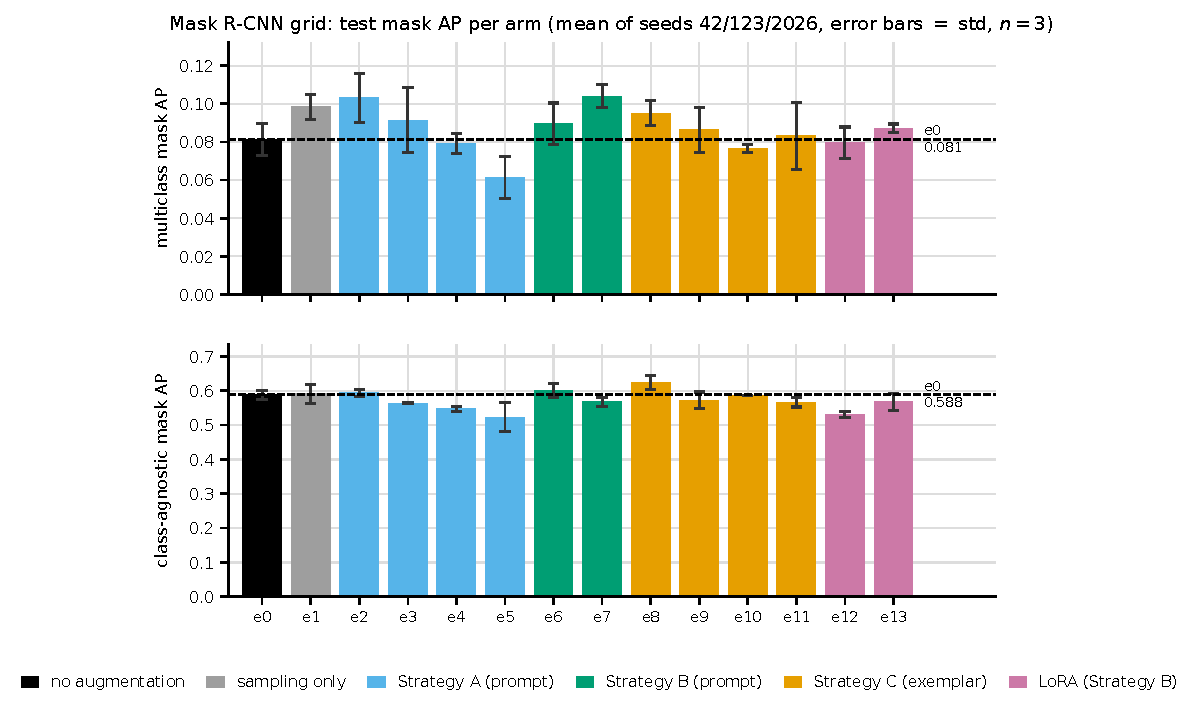
\includegraphics[width=\textwidth]{images/fig_grid_ap.pdf}
\caption{Mask R-CNN grid: mask AP per arm in both tracks.}
\label{fig:gridap}
\end{figure}

The class-agnostic track is the more legible half of the grid, because its
standard deviations are proportionally much smaller. The baseline is
$0.588 \pm 0.013$. The best arm is copy-paste at $0.624 \pm 0.020$, a difference
of $+0.036$ with all three seeds positive; the worst is the LoRA conversion at
$0.531 \pm 0.010$, a difference of $-0.057$ with all three seeds negative. Nine
of the thirteen augmented arms fall below the baseline: e3, e4, e5, e7, e9, e10,
e11, e12 and e13. Only e1, e2, e6 and e8 are above it. Every paired sign test
again returns $p \ge 0.25$, so none of these differences --- including the
$+0.036$ of copy-paste and the $-0.057$ of LoRA --- meets a conventional
significance threshold at this sample size. What the pattern does support is a
directional statement that does not depend on any single test: the arms that add
diffusion-generated pixels (e2--e5, e10--e13) are distributed around and mostly
below the baseline, and the one arm that adds only real transplanted pixels is
the highest.

Rare-class macro AP, the quantity the entire augmentation effort was designed to
raise, is effectively zero everywhere. The largest value in the grid is $0.0036$
for copy-paste, and its three seeds are $\{0.0108, 0.0000, 0.0000\}$ --- a single
seed in which one rare instance happened to be matched. The paired test on this
metric returns $p = 1.00$. Six of the fourteen arms score exactly $0.0000$.
Figure~\ref{fig:raremacro} plots these values on an axis scaled to the
class-agnostic baseline, which is the clearest single statement of the project's
outcome: the bars are invisible.

\begin{figure}[H]
\centering
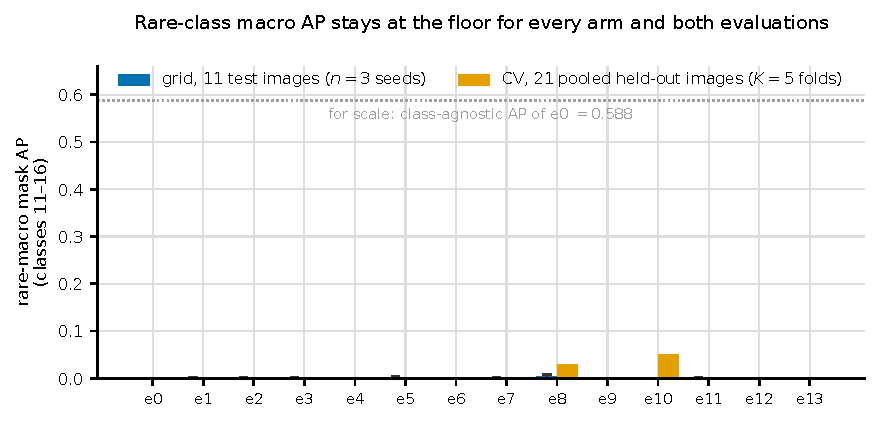
\includegraphics[width=\textwidth]{images/fig_rare_macro.pdf}
\caption{Rare-class macro AP across arms and both evaluations.}
\label{fig:raremacro}
\end{figure}

\subsection*{Experiment 2: rotated held-out cross-validation}

The grid's test split is 11 images. The cross-validation re-evaluates the frozen
grid checkpoints on five disjoint folds of the 21 held-out images, so every
held-out image is scored exactly once and the pooled rare support rises from 17
to 40 instances. Results for the six selected arms are in Table~\ref{tab:cv}.

\begin{table}[H]
\centering
\caption{Rotated held-out cross-validation, $K=5$ folds over 21 held-out images,
evaluation-only on the frozen grid checkpoints. Mean $\pm$ std over folds;
``pos.\ folds'' counts folds in which the arm exceeded e0; $p$ is the exact
two-sided paired sign test over folds, whose minimum attainable value at $K=5$ is
$0.0625$. Source: \protect\path{outputs/final/cv/summary.csv} and \texttt{summary.json}.}
\label{tab:cv}
\small
\begin{tabular}{@{}ll rrrr r rrr@{}}
\toprule
& & \multicolumn{4}{c}{Multiclass overall AP} & rare & \multicolumn{3}{c}{Class-agnostic overall AP} \\
\cmidrule(lr){3-6}\cmidrule(lr){7-7}\cmidrule(lr){8-10}
Arm & Method & AP & $\Delta$ & pos. & $p$ & macro AP & AP & $\Delta$ & pos. \\
\midrule
e0  & Original            & $0.143 \pm 0.037$ & ---      & ---  & ---   & $0.000$ & $0.602 \pm 0.044$ & ---      & --- \\
e1  & Rare-weighted       & $0.154 \pm 0.019$ & $+0.011$ & 3/5  & 1.000 & $0.000$ & $0.615 \pm 0.072$ & $+0.013$ & 3/5 \\
e6  & Strategy B          & $0.153 \pm 0.013$ & $+0.010$ & 2/5  & 1.000 & $0.000$ & $0.626 \pm 0.060$ & $+0.024$ & 4/5 \\
e8  & C copy-paste        & $0.152 \pm 0.020$ & $+0.010$ & 4/5  & 0.375 & $0.029$ & $\mathbf{0.647 \pm 0.061}$ & $+0.045$ & \textbf{5/5} \\
e10 & C diffusion inpaint & $0.135 \pm 0.032$ & $-0.008$ & 2/5  & 1.000 & $0.050$ & $0.616 \pm 0.061$ & $+0.014$ & 3/5 \\
e12 & LoRA Strategy B     & $0.134 \pm 0.020$ & $-0.008$ & 3/5  & 1.000 & $0.000$ & $0.568 \pm 0.077$ & $-0.034$ & 1/5 \\
\bottomrule
\end{tabular}
\end{table}

The multiclass picture is unchanged: the six arms span $0.134$ to $0.154$ against
a baseline of $0.143 \pm 0.037$, the two diffusion-based arms (e10, e12) are the
two lowest, and no paired test falls below $p = 0.375$. Overall AP is roughly
twice its grid value in every arm, which reflects the different composition of
the evaluation set rather than any change in the models --- the folds include the
former validation images, which are drawn from a project whose plans the
detectors find easier.

The class-agnostic column contains the one result in the project with a
consistent sign. Copy-paste scores $0.647 \pm 0.061$ against $0.602 \pm 0.044$,
a difference of $+0.045$ that is positive in all five folds
($\{+0.070, +0.033, +0.016, +0.040, +0.067\}$). The exact two-sided sign test
gives $p = 0.0625$, which is the smallest value obtainable with $K = 5$ and
therefore does not clear $0.05$ no matter how consistent the effect is. This is a
limit of the design, not of the result, and it is stated as such: five folds
cannot produce a conventionally significant two-sided sign test. The remaining
class-agnostic arms are further from significance still: $p = 1.000$ for e1 and
e10, $p = 0.375$ for e6 and for e12's negative $-0.034$. The honest summary is
that copy-paste shows a small positive effect that replicated across every fold
and across both Mask R-CNN evaluations, and that the evidence is suggestive
rather than conclusive. Figure~\ref{fig:cvagnostic} shows the fold
structure directly.

\begin{figure}[H]
\centering
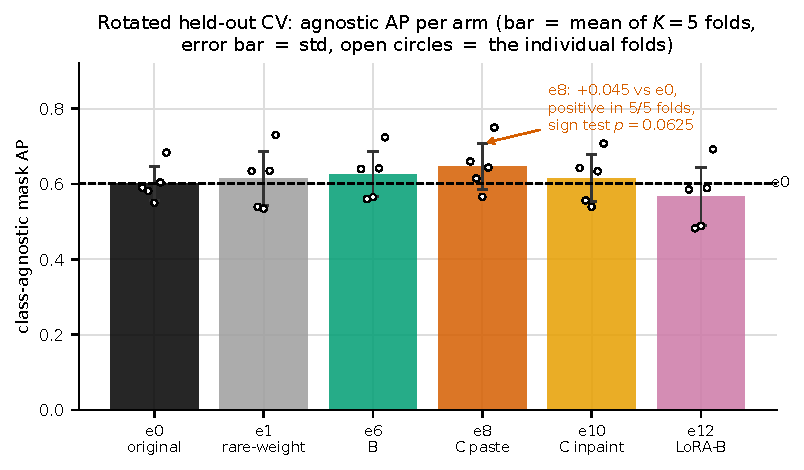
\includegraphics[width=\textwidth]{images/fig_cv_agnostic.pdf}
\caption{Cross-validation: class-agnostic AP per arm with per-fold points.}
\label{fig:cvagnostic}
\end{figure}

Pooling the folds also gives the first non-zero rare numbers in the project, and
they are worth stating precisely because they look better than they are. The
pooled rare-macro AP is $0.050$ for e10 and $0.029$ for e8, against $0.000$ for
e0, e1, e6 and e12. In both cases the entire value comes from a single category:
Abstellraum (class 12, pooled support 3 instances), which reaches a pooled mask
AP of $0.300$ for e10 and $0.176$ for e8. The other five primary-rare categories
score exactly $0.000$ in every arm, including Allg.\ Verkehrsfl\"ache with the
largest pooled rare support of 13 instances. A rare-macro AP of $0.05$ driven by
three instances of one class is not evidence that inpainting augmentation
improves rare-class segmentation.

\subsection*{Experiment 3: SAM 3}

Table~\ref{tab:sam3} gives the SAM 3 runs alongside the matched Mask R-CNN arms,
and Figure~\ref{fig:sam3} plots the comparison. Each SAM 3 cell is a single
training run; the Mask R-CNN cells are means over three seeds with their standard
deviations, which is what makes the comparison interpretable.

\begin{table}[H]
\centering
\caption{SAM 3 versus Mask R-CNN on the same test split and the same augmented
datasets. SAM 3 values are single runs ($n=1$, no std available); Mask R-CNN
values are mean $\pm$ std over three seeds. Sources:
\protect\path{outputs/final/sam3/summary.csv} and
\protect\path{outputs/final/grid_r1/summary.csv}.}
\label{tab:sam3}
\small
\begin{tabular}{@{}ll rr rr@{}}
\toprule
& & \multicolumn{2}{c}{Multiclass mask AP} & \multicolumn{2}{c}{Class-agnostic mask AP} \\
\cmidrule(lr){3-4}\cmidrule(lr){5-6}
Training data & Arm & SAM 3 ($n{=}1$) & Mask R-CNN ($n{=}3$) & SAM 3 ($n{=}1$) & Mask R-CNN ($n{=}3$) \\
\midrule
Original (no aug)    & e0  & $0.115$ & $0.081 \pm 0.008$ & $\mathbf{0.713}$ & $0.588 \pm 0.013$ \\
C diffusion inpaint  & e10 & $0.120$ & $0.077 \pm 0.002$ & $0.704$ & $0.586 \pm 0.001$ \\
LoRA Strategy B      & e12 & $0.140$ & $0.080 \pm 0.008$ & $0.685$ & $0.531 \pm 0.010$ \\
C copy-paste         & e8  & $\mathbf{0.147}$ & $0.095 \pm 0.007$ & $0.693$ & $0.624 \pm 0.020$ \\
\midrule
\multicolumn{2}{@{}l}{$\Delta$ vs.\ own baseline, best aug.} & $+0.032$ & $+0.014$ & $-0.009$ & $+0.036$ \\
\bottomrule
\end{tabular}
\end{table}

\begin{figure}[H]
\centering
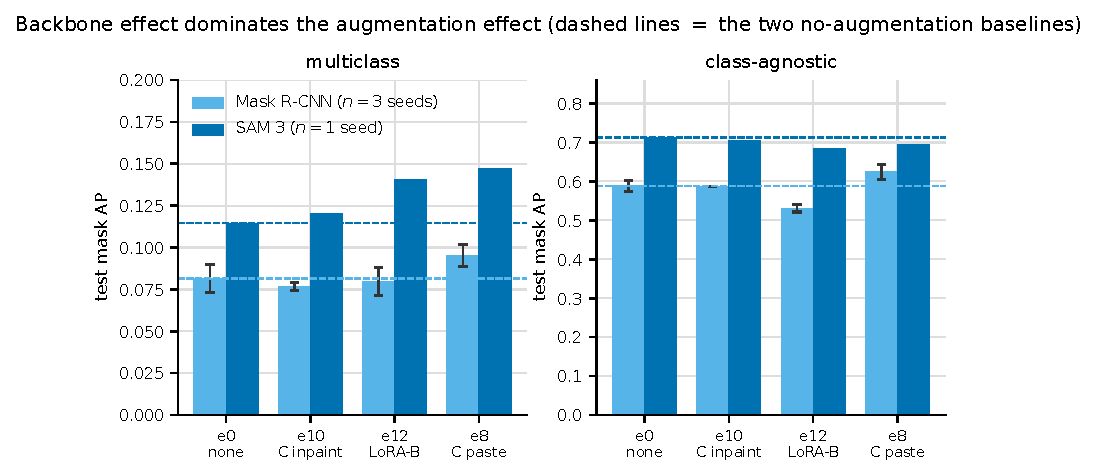
\includegraphics[width=\textwidth]{images/fig_sam3_vs_mrcnn.pdf}
\caption{SAM 3 against Mask R-CNN, baseline and augmented, in both tracks.}
\label{fig:sam3}
\end{figure}

On the multiclass track SAM 3 improved under all three augmentations: $+0.005$
for diffusion inpaint, $+0.026$ for the LoRA conversion and $+0.032$ for
copy-paste, the last being the largest positive augmentation effect measured
anywhere in the project. It is nevertheless not evidence of an effect. Each value
is a single run, and the seed-to-seed standard deviation measured on the Mask
R-CNN multiclass grid ranges from $0.002$ to $0.018$, with individual arms
spanning up to $0.031$ across their three seeds. All three SAM 3 deltas lie
inside that band, so a plausible alternative explanation is that they are the
draw of one seed. Reporting them as improvements would require the three-seed
repetition that queue time did not allow.

On the class-agnostic track the direction reverses: every augmentation lowered
SAM 3's AP, from $0.713$ at baseline to $0.704$, $0.693$ and $0.685$. The sign
of the copy-paste effect is therefore opposite in the two backbones ($+0.036$ for
Mask R-CNN, $-0.020$ for SAM 3), which is itself an argument against reading any
of these single-run deltas as a property of the augmentation.

The one comparison in Table~\ref{tab:sam3} that is not fragile is the vertical
one. SAM 3's unaugmented class-agnostic AP of $0.713$ exceeds the best Mask R-CNN
arm ($0.624$ for e8) by $0.089$, and its unaugmented multiclass AP of $0.115$
exceeds the best Mask R-CNN arm ($0.104$ for e7) by $0.011$. The class-agnostic
gap is roughly two and a half times the largest augmentation delta measured in
the entire grid and an order of magnitude above the typical one. Whatever benefit
augmentation might carry at this data scale, backbone choice dominates it.

\subsection*{Experiment 4: the two-stage DINOv2 pipeline}

Stage 2 was trained on 887 real training crops, optionally extended with the 171
synthetic rare crops produced by the augmentation pipeline, and evaluated both on
368 real ground-truth test crops (Evaluation A) and end-to-end over 483
class-agnostic SAM 3 test proposals (Evaluation B). Table~\ref{tab:dino} gives
both.

\begin{table}[H]
\centering
\caption{Two-stage room typing with a frozen DINOv2-base encoder.
Evaluation A classifies 368 ground-truth test crops, removing detector error;
Evaluation B labels 483 class-agnostic SAM 3 proposals and scores the result as
multiclass instance segmentation on the same test split as every other
experiment. Single runs. Source: \protect\path{outputs/final/dino/summary.csv} and
\texttt{report.md}.}
\label{tab:dino}
\small
\begin{tabular}{@{}ll rrr rr@{}}
\toprule
& & \multicolumn{3}{c}{Evaluation A: GT-crop classification} & \multicolumn{2}{c}{Evaluation B: two-stage} \\
\cmidrule(lr){3-5}\cmidrule(lr){6-7}
Head training set & Head & top-1 & head-macro rec. & rare-macro rec. & mask AP & rare AP \\
\midrule
real (887 crops)          & linear & $\mathbf{0.454}$ & $\mathbf{0.381}$ & $0.000$ & $\mathbf{0.0910}$ & $0.0000$ \\
real (887 crops)          & kNN    & $0.386$ & $0.332$ & $0.000$ & $0.0797$ & $0.0000$ \\
real $+$ 171 synth.\ rare & linear & $0.440$ & $0.354$ & $0.000$ & $0.0892$ & $0.0000$ \\
real $+$ 171 synth.\ rare & kNN    & $0.340$ & $0.286$ & $0.000$ & $0.0748$ & $0.0042$ \\
\midrule
\multicolumn{5}{@{}l}{\emph{reference, end-to-end fine-tuned, same test split:} SAM 3 multiclass} & $0.115$ & \\
\multicolumn{5}{@{}l}{\emph{reference:} best Mask R-CNN arm (e7, $n{=}3$)} & $0.104$ & \\
\multicolumn{5}{@{}l}{\emph{reference:} Mask R-CNN e0 ($n{=}3$)} & $0.081$ & \\
\bottomrule
\end{tabular}
\end{table}

Evaluation A is the diagnostic result of the project. Given perfect
ground-truth crops --- no detector error at all --- a frozen DINOv2-base encoder
with a linear head reaches $0.454$ top-1 over 19 classes and $0.381$ macro recall
over the ten head classes, but $0.000$ macro recall over the six primary-rare
classes. That zero holds in every arm and for both heads. Figure~\ref{fig:dinorecall}
shows the per-class breakdown: recall is $0.96$ for Treppe, $0.82$ for WC and
$0.69$ for Aufzug, then collapses --- $0.15$ for Lager, $0.08$ for Technikraum,
and exactly zero for K\"uche, ``Flur, Halle'', Besprechungsraum and all six rare
classes. Since localisation is not involved, this locates the failure squarely in
room-type classification, and it shows that the failure is not confined to the
tail: four head classes with 3--16 test instances also score zero.

\begin{figure}[H]
\centering
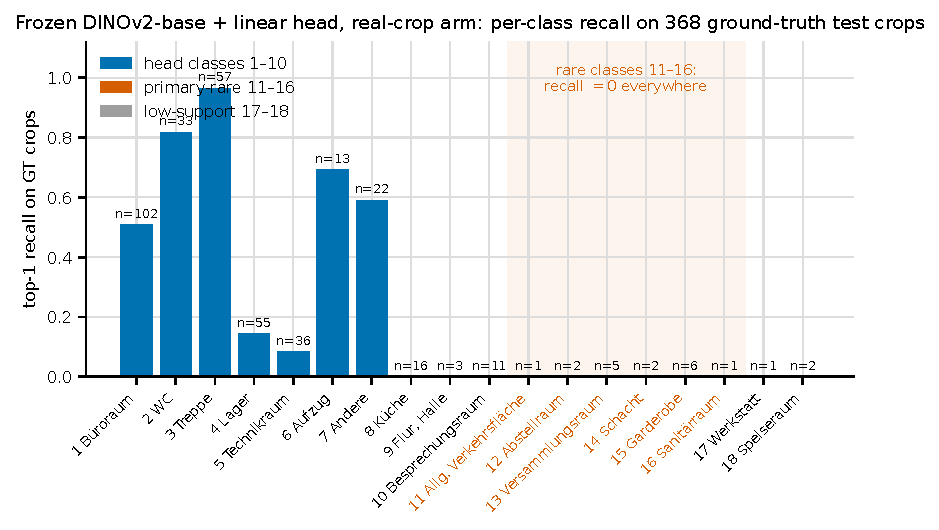
\includegraphics[width=\textwidth]{images/fig_dino_recall.pdf}
\caption{Per-class recall of the frozen DINOv2 classifier on ground-truth crops.}
\label{fig:dinorecall}
\end{figure}

Adding the 171 synthetic rare crops did not help. Top-1 accuracy fell from
$0.454$ to $0.440$ for the linear head and from $0.386$ to $0.340$ for kNN,
head-macro recall fell in both, and rare-macro recall stayed at $0.000$. The
synthetic crops were produced by the same pipeline whose output the detectors
also declined to benefit from, so the result is consistent rather than
surprising, but it closes off the hypothesis that the crops were useful data that
the detector setting simply failed to exploit. The single non-zero rare number in
the whole table --- a two-stage rare AP of $0.0042$ for the real-plus-synthetic
kNN arm --- comes from an arm whose overall accuracy is the worst of the four and
whose rare-macro recall is still zero.

Evaluation B places the pipeline on the same axis as the fine-tuned detectors.
Its best configuration reaches $0.0910$ two-stage mask AP, below fine-tuned SAM 3
($0.115$) and below the best Mask R-CNN arm ($0.104$), and above only the
unaugmented Mask R-CNN baseline ($0.081$). Figure~\ref{fig:dinotwostage} shows
this against the three reference lines. Decomposing the problem therefore did not
recover the accuracy that end-to-end fine-tuning achieves, even though stage 1 is
the strongest localiser available: SAM 3 finds room boundaries at $0.713$
class-agnostic AP, and the two-stage system converts that into $0.091$ multiclass
AP. The gap between those two numbers is the classification problem, measured
end-to-end.

\begin{figure}[H]
\centering
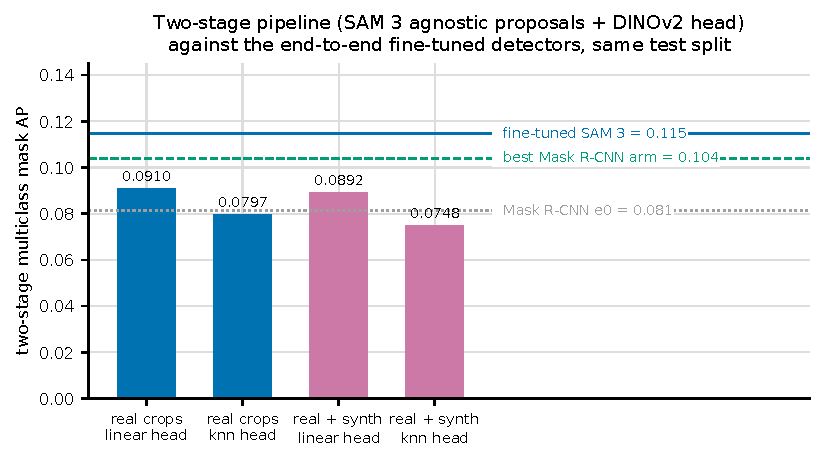
\includegraphics[width=\textwidth]{images/fig_dino_twostage.pdf}
\caption{Two-stage mask AP against the end-to-end fine-tuned detectors.}
\label{fig:dinotwostage}
\end{figure}

\subsection*{Qualitative check}

Figure~\ref{fig:predmulticlass} pairs ground truth with the multiclass Mask R-CNN
prediction on test plan 034, and Figure~\ref{fig:predagnostic} does the same for
the class-agnostic model. The contrast is the numerical result made visible. The
class-agnostic model recovers nearly every room polygon in the plan, including
the small service rooms along the perimeter. The multiclass model on the same
image recovers the corridor network and the two Luftr\"aume, but leaves a large
share of the offices, the meeting rooms and the Abstellraum in the upper left
uncoloured, and predicts no rare-class instance anywhere on the plan. The two
panels differ only in the label space of the model that produced them. This is
the same story as
Tables~\ref{tab:grid}--\ref{tab:dino}: the geometry is available and the label is
not.

\begin{figure}[H]
\centering
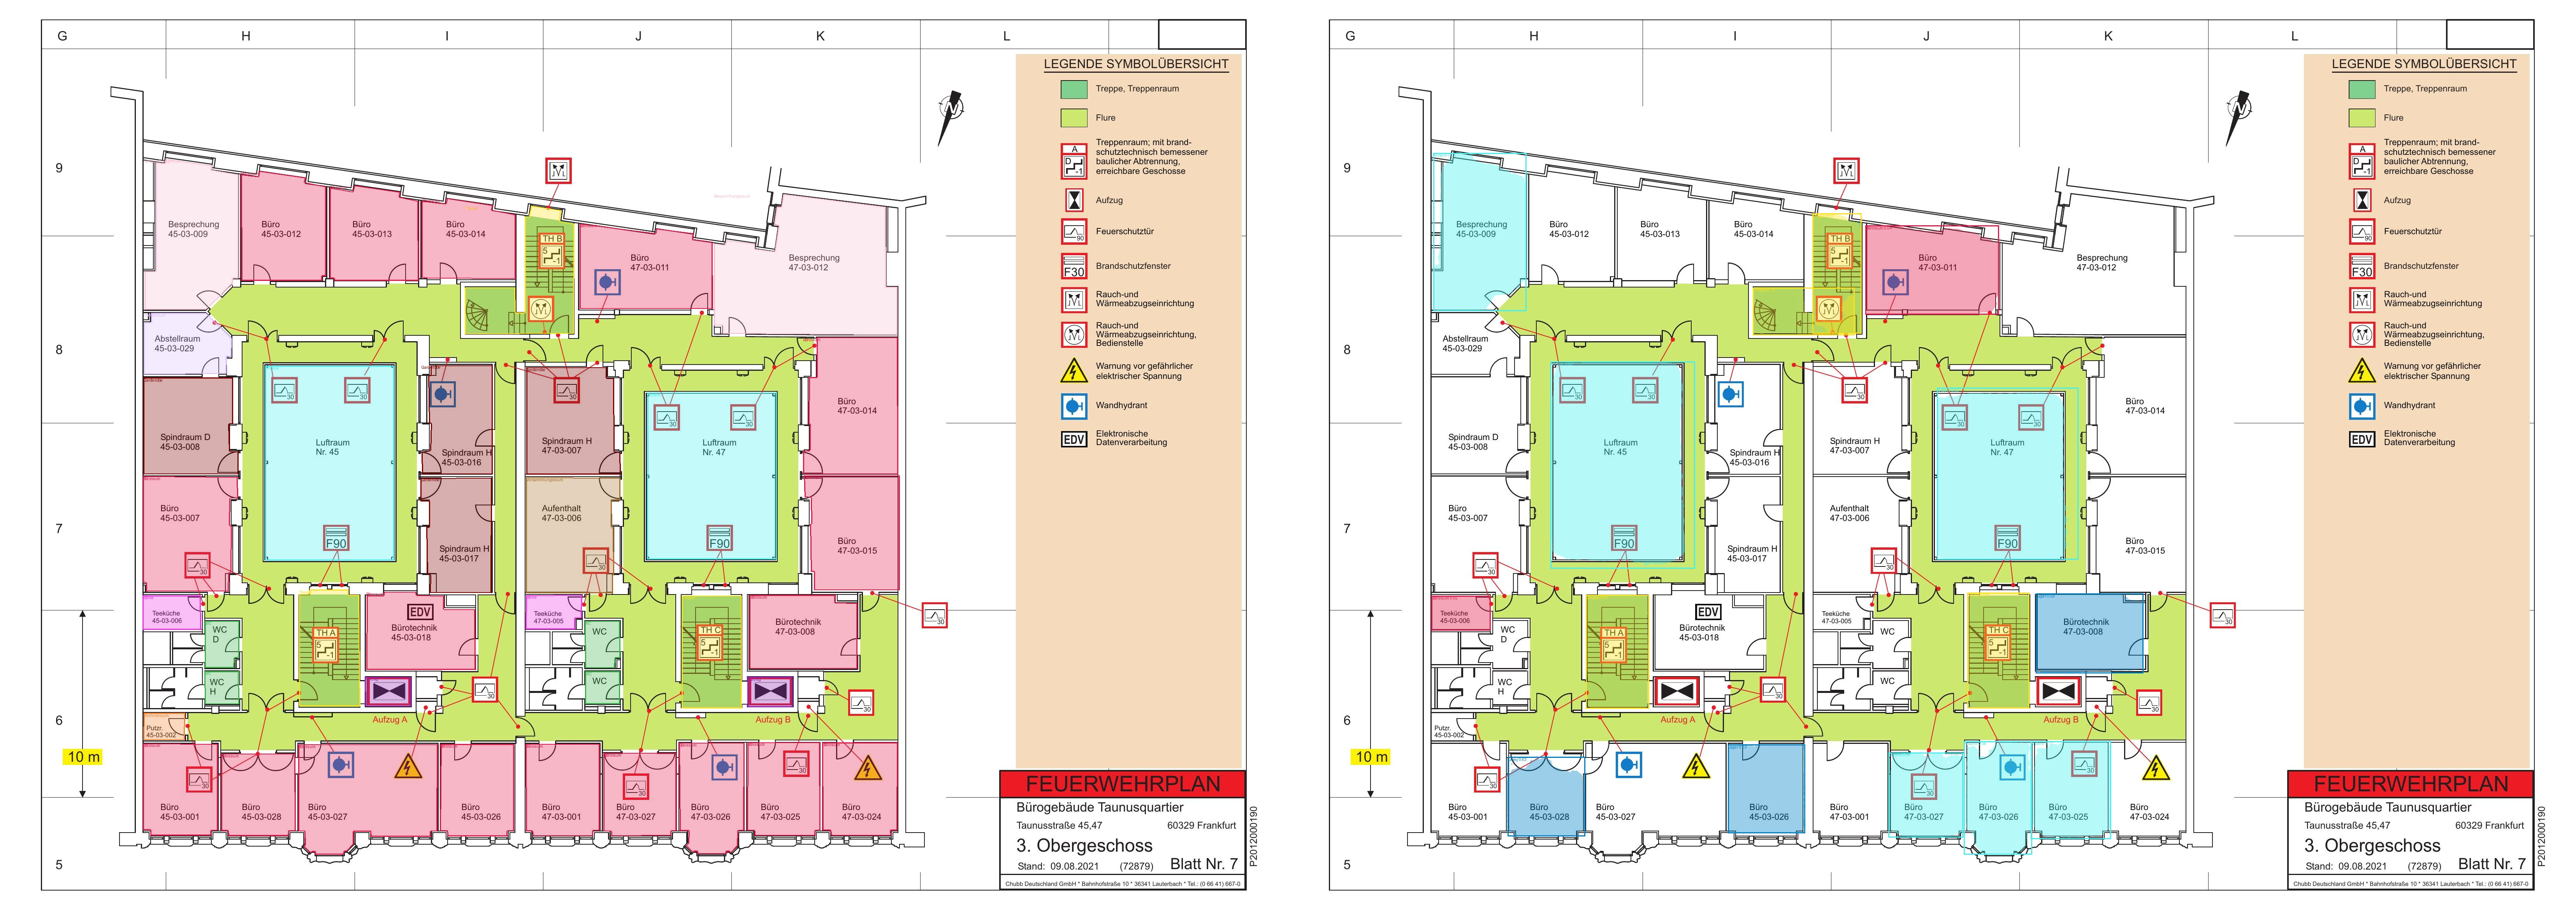
\includegraphics[width=\textwidth]{images/mrcnn_multiclass_034.jpg}
\caption{Multiclass Mask R-CNN: ground truth (left) versus prediction (right).}
\label{fig:predmulticlass}
\end{figure}

\begin{figure}[H]
\centering
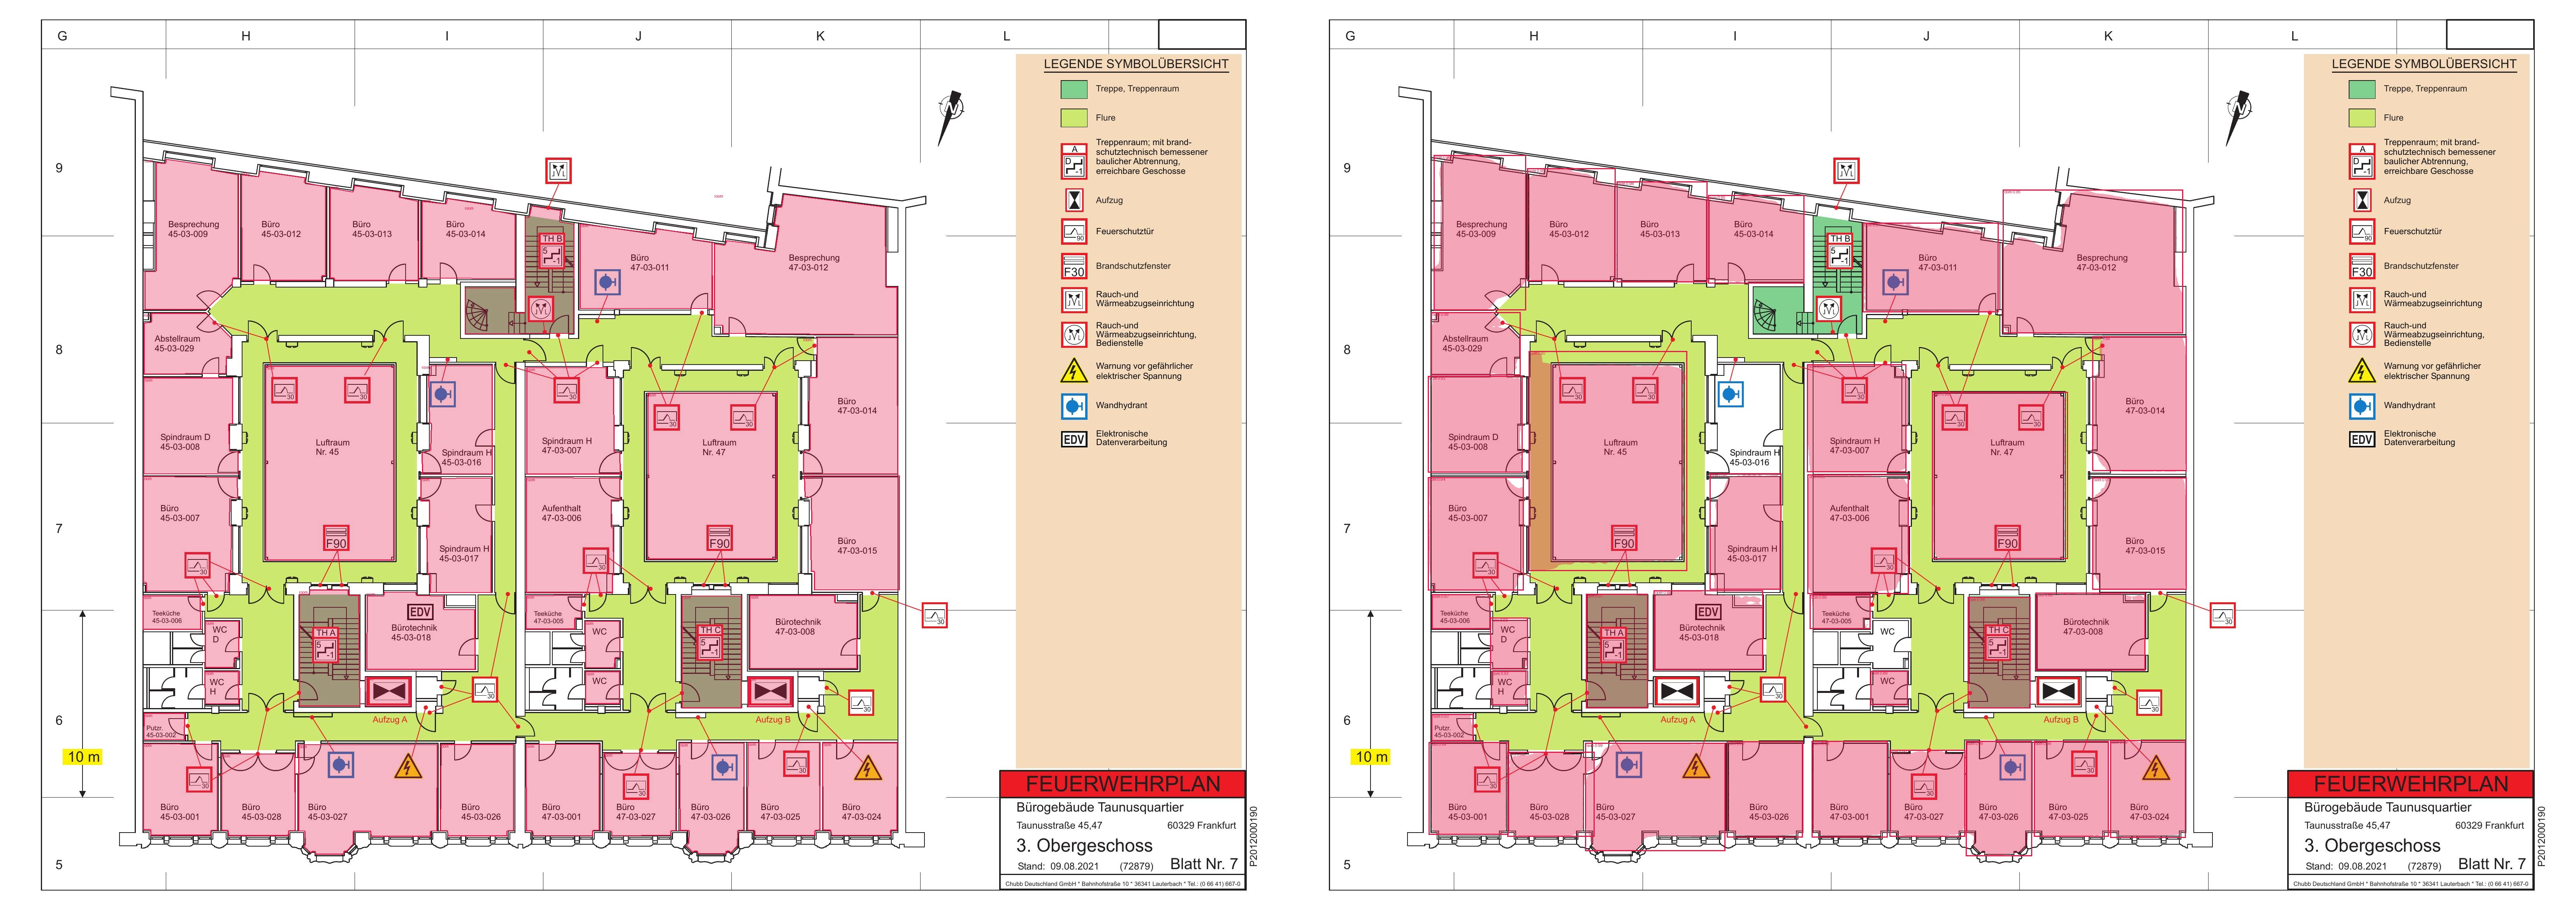
\includegraphics[width=\textwidth]{images/mrcnn_agnostic_034.jpg}
\caption{Class-agnostic Mask R-CNN on the same test plan.}
\label{fig:predagnostic}
\end{figure}

\subsection*{Summary of the evidence}

Reading the four experiments together, three statements are supported and one
frequently-made statement is not.

Diffusion and LoRA inpainting augmentation did not reliably improve floor-plan
room segmentation. On Mask R-CNN the effect is neutral to harmful and replicated
as such across three seeds and five cross-validation folds: nine of thirteen
augmented arms fall below baseline on the class-agnostic grid, the two
diffusion-based arms are the two lowest multiclass arms in the cross-validation,
and the LoRA arm is the worst arm in the grid at $-0.057$. On SAM 3 there is a
small multiclass gain that is unreplicated, single-seed, and inside the noise
band measured on the grid, accompanied by a class-agnostic loss under every
augmentation. As classifier-crop augmentation the synthetic data lowered every
metric it touched.

Simple exemplar copy-paste --- the control arm containing no generated pixels ---
is the only augmentation with a small, consistent positive effect. It is the
top-ranked arm in three of the six backbone $\times$ track comparisons run in the
project (Mask R-CNN class-agnostic grid, Mask R-CNN class-agnostic
cross-validation, SAM 3 multiclass); it is not top-ranked in the Mask R-CNN
multiclass grid (e7 leads), the multiclass cross-validation (e1 leads), or the
SAM 3 class-agnostic track (the baseline leads). Its strongest single result is
the cross-validated $+0.045$ class-agnostic AP, positive in all five folds at
$p = 0.0625$.

The backbone dominates the augmentation. SAM 3 exceeds the best Mask R-CNN arm by
$0.089$ class-agnostic AP and $0.011$ multiclass AP without any augmentation at
all, and the class-agnostic figure is larger than every augmentation delta
measured in the project.

What is not supported is the premise the project set out to test. Rare-class room
segmentation is not merely unimproved by augmentation; it is out of reach at this
data scale by any method tried. Rare AP is at or near zero across all fourteen
arms, both backbones and both evaluation protocols, and rare-macro recall is
exactly zero even when a frozen classifier is handed perfect ground-truth crops.
With 17 rare test instances --- 40 when pooled over the cross-validation --- the
experiment can exclude a large effect and cannot resolve a small one. Meanwhile
class-agnostic localisation already works, at $0.588$--$0.647$ AP for Mask R-CNN
and $0.713$ for SAM 3. The unsolved component is room-type classification, and a
dedicated frozen classifier did not fix it.
